\chapter{Cloud Security with Honeypots}

In this chapter we investigate... tbc.

\section{Introduction}

As previously mention in \fullref{sec:cloud-computing}, using cloud resources are becoming the go-to option for new services, and applications.
\citet{Kelly2021} thoroughly investigated honeypots on cloud providers such as Azure, \ac{aws}, or \ac{gcp}.
Followingly, we present their results that we want to compare with the results of heiCLOUD later on.
The results are collected by T-Pot version $20.06.0.$ over a duration of 3 weeks.
In addition, \citet{Kelly2021} considered different server geographical locations.
They have collected data from East US, West Europe, and Southeast Asia.
\autoref{tab:overview-cloud-security} shows the results presented by \citet{Kelly2021}.
Dionaea (a honeypot to capture malicious payload), Cowire (SSH and Telnet honeypot), and Conpot (industrial honeypot for \ac{ics}, and \ac{scada}) are the most attacked honeypots in comparison to the others.
Regarding \ac{aws}, Dionaea account $91\%$ of the total attacks, Glutton and Cowire are minor with $5\%$, and $2\%$.
Interestingly, Cowire reported several attacks related to the COVID-19 pandemic to enable social engineering methods.
In contrast to \ac{aws}, Cowire logged the majority of attacks with $51\%$ on \ac{gcp}.
Beside several automated attacks trying to login with default credentials, adversaries tried to gather information about CPU architecture, scheduled tasks, and privilege escalation.
Microsoft Azure reflects nearly the same results as the other two cloud providers beforehand.

\begin{table}
    \centering
    \caption[Overview of attacks on cloud providers]{Overview of attacks on cloud providers. For a better overview, only the three most attacked honeypots are listed. The others combine several honeypots.}
    \begin{tabularx}{\linewidth}{l|XXXX|l}
        \toprule
        \textsc{Provider} & \multicolumn{4}{c|}{\textsc{Honeypot}} & \textsc{In Total}                                                  \\
                          & \textbf{Dionaea}                       & \textbf{Cowire}   & \textbf{Glutton} & \textbf{others} &           \\
        \hline
        \acl{aws}         & $228.075$                              & $4.503$           & $11.878$         & $3.688$         & $248.144$ \\
        \acl{gcp}         & $162.570$                              & $297.818$         & $84.375$         & $36.403$        & $581.116$ \\
        Microsoft Azure   & $308.102$                              & $9.012$           & $17.256$         & $6.365$         & $340.735$ \\
        \bottomrule
    \end{tabularx}
    \label{tab:overview-cloud-security}
\end{table}

The overall results show an average ratio of $55.000$ attacks per day, summing up to roughly $1.6$ mio in total.
Similar results for different regions could have been reprocuded.
Their results clearly show the disparity of the regions Europe, US, and Asia.
An important question that \citet{Kelly2021} answered is if attackers target services on cloud providers based on the cloud providers' market share.
They could not confirm this assumption based on the fact that Google Cloud with the smallest market share received most of the attacks.
In total, most of the attacks are originated from Vietnam, Russia, United States, and China.
Due to technologies such as VPN, or Tor, the geolocation only indicates the last node, so location data might be distorted.
Across all providers roughly $80\%$ of the source IP addresses had a bad reputation and could been filtered by the organization.
The operating devices used for attacking the services are mostly Windows 7 or 8, and different Linux kernels and distributions.
Windows devices target vulnerabilities in remote desktop sharing software. Such vulnerabilities are
\begin{enumerate*}[label=(\roman*)]
    \item CVE-2006-2369\cite{CVE-2006-2369} (RealVNC) in the US region,
    \item CVE-2001-0540\cite{CVE-2001-0540} (RDP) in EU and Asia regions,
    \item CVE-2012-0152\cite{CVE-2012-0152} (RDP) in the Asia region, and
    \item CVE-2005-4050\cite{CVE-2005-4050} (VoIP) in EU region
\end{enumerate*}.
In addition, attackers were also capable of disguising any fingerprinting activity of p0f.

In this chapter, we want to compare the findings \citet{Kelly2021} claimed in the paper \enquote{A Comparative Analysis of Honeypots on Different
    Cloud Platforms} with ours using the University Heidelberg's cloud solution.
First, a short introduction of heiCLOUD is held, followed by a closer lookup of T-Pot that is used to acquire data.
Lastly, we present the results and do a thorough comparison closing up with a discussion based on a technical report of the Campridge University.

\section{Methodology}

Our foremost goal is to track as most attacks as possible.
To gather various attacks from the Internet \autoref{fig:concept} sketches our concept we plan to apply.
Honeypots should be deployed on a single instance, and store their data, or log files in a database.
By the help of data visualization tools we analyze the attacks.
For security reasons, honeypots should run in virtualized environment to avoid any harm to our host system.
We use Debian as a base linux distribution.
Our instance runs on heiCLOUD, a cloud service provided by Heidelberg University.
It is capable of 16 GB of RAM, 8 VCPUs, and a volatile memory of 30 GB.
In addition, we mount a 125 GB permanent memory to securily store our data.
In its very early stages, we compared different approaches to achieve this goal.
As an example we compared native implementation approaches, using additional frameworks, and ready-to-use solutions.
However, the T-Pot , developed by Telekom, offers a profoundly ready-to-use solution with major advantages.
It combines several honeypots in conjunction with various analytic tools to trace the newest attacks.
In addition, it helps to compare our findings with the ones \citet{Kelly2021} claims.

\begin{figure}[h]
    \centering
    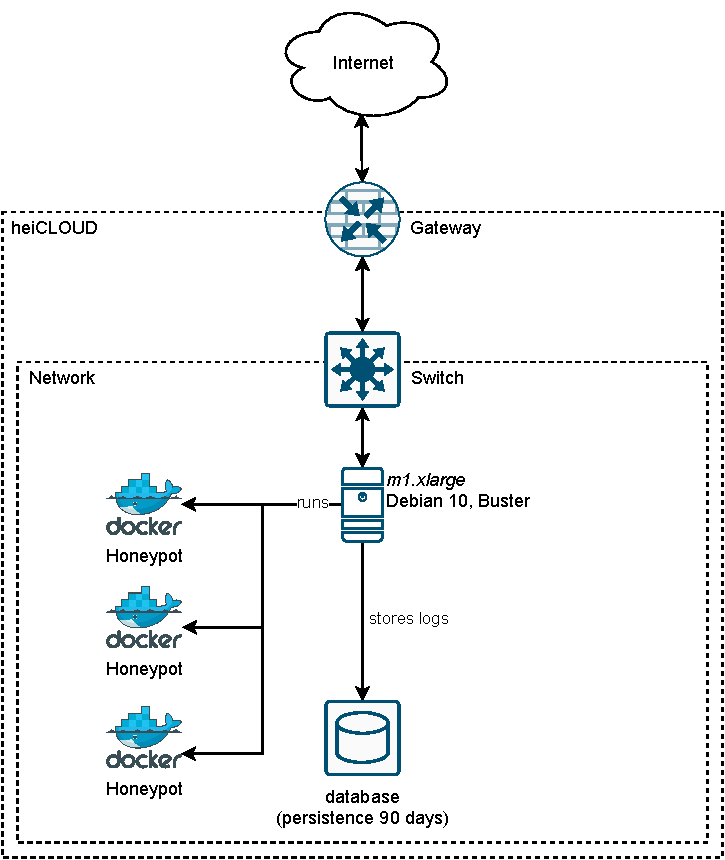
\includegraphics{figures/tpot-concept.pdf}
    \caption[Draft for data collection]{Concept to collect honeypot attacks}
    \label{fig:concept}
\end{figure}

Running our instance and exposing it to the Internet needs some adjustments beforehand.
Therefore, a virtual network with subnet \ipAddress{192.168.145.0/24} has been created wherein our instance with IP address \ipAddress{192.168.145.4} is assigned to.
The instance is accessible from the outside with floating IP address \ipAddress{129.206.5.74}.
Access rules are similar to a stateful firewall, and thus, do not block any attacks.
Ports $1-64000$ are exposed and can be attacked by anyone.
Ports higher than $64000$ are only accessible through the University network \ipAddress{129.206.0.0/16} or eduroam \ipAddress{147.142.0.0/16} and should provide a basic authentication with username and password.

\subsection{heiCLOUD}
\label{subsec:heicloud}

\citet{urz2021} offers a \enquote{\ac{iaas} specially tailored for higher education and research institutions} called heiCLOUD.
It supplies multiple institutes at University Heidelberg with storage, virtual machines, or network components.
In addition, heiCLOUD is a DFN\footnote{German National Research and Education Network,  the communications network for Science and research in Germany} member, and offers others to use their services.
As stated on their information website\cite{heicloud2021}, it is
\begin{enumerate*}[label=(\roman*)]
    \item capable of freely manageable IT resources,
    \item beholds a stable and fast connection,
    \item ensures high availability and scalability,
    \item has freely selectable VM operating systems, and
    \item has a transparent payment model
\end{enumerate*} \cite{heicloud2021}.
Based on the open source application OpenStack, users can easily create own network areas, and manage their space individually.
Unlike well-known cloud providers, heiCLOUD servers are located withing Germany, thus, abide by the European data privacy law.
HeiCLOUD have never considered honeypots for additional cyber security measurements.

\subsection{T-Pot}
\label{subsec:tpot}

To be able to compare our results with \citet{Kelly2021}, we use the same approach to capture recent cyber attacks.
The T-Pot solution, a mixture of Telekom and Honeypot, stands out with their sheer quantity of various honeypots.
It requires $8$ GB RAM and a minimum of $128$ GB hard drive storage.
Based on a Debian 10 Buster distribution, it relies on Docker to run their services \cite{docker2021}.
T-Pot has to be deployed in a reachable network where intruders are expected.
Either TCP and UDP traffic are forwarded without filtering to the network interface, or it runs behind a firewall with forwarding rules.
Specified ports for attackers are $1$-$64000$, higher ports are reserved for trusted IPs, thus, a reverse proxy asks for basic authentication.
All daemons and tools run on the same network interface whereas some of them are encapsulated in their own Docker network.
Docker is a lightweight virtualization technology that uses containers to run on the host system \cite{combe2016}.
Unlike virtual machines, Docker reduces overhead with the downside of a greater attack surface.
To mitigate attacks, Docker wraps containers in an isolated environment.
This is achieved by restricting the kernel namespace and control groups (cgroups).
\autoref{fig:overview-tpot} visualizes the technical concept of T-Pot.
Each service has dedicated ports or port ranges that are exposed.
Attackers can communicate either with TCP or UDP.
All honeypots and tools create log files that are used to get any knowledge about attackers.
In order to view and trace current attacks, T-Pot uses the ELK stack.
ELK is the acronym of Elasticsearch, Logstash and Kibana \cite{elastic2021}.
Elasticsearch is a search engine based on Lucene.
It is multitenat-capable and offers full-text search via HTTP.
Logstash is used to feed elasticsearch.
In general, it offers a open server-side data processing pipeline that helps to send data from multiple sources to an elasticsearch node.
Kibana is the main data visualization tool.
It offers users to create plots and dashboards, crawl elasticsearch, and trace the system health.
All logs of the honeypots and tools are forwarded to the search engine Elasticsearch by Logstash.
The ELK stack is not directly exposed to the Internet, thus, an authentication is not needed.
Users can monitor all logfiles with Kibana by pre-defined dashboards, or custom search queries.
In addition, T-Pot features different services types, namely
\begin{enumerate*}[label=(\roman*)]
    \item standard,
    \item sensor,
    \item industrial,
    \item collector,
    \item next generation, and
    \item medical
\end{enumerate*}.
Each service type has a different set of honeypots and tools tailored to their core idea.
T-Pot feeds their data to an external Telekom service, however, this data submission can be turned off.
For this chapter we restrict ourself to the latest version $20.06.0$.
Newer versions might be available by time and could differ from ours.

\begin{sidewaysfigure}
    \centering
    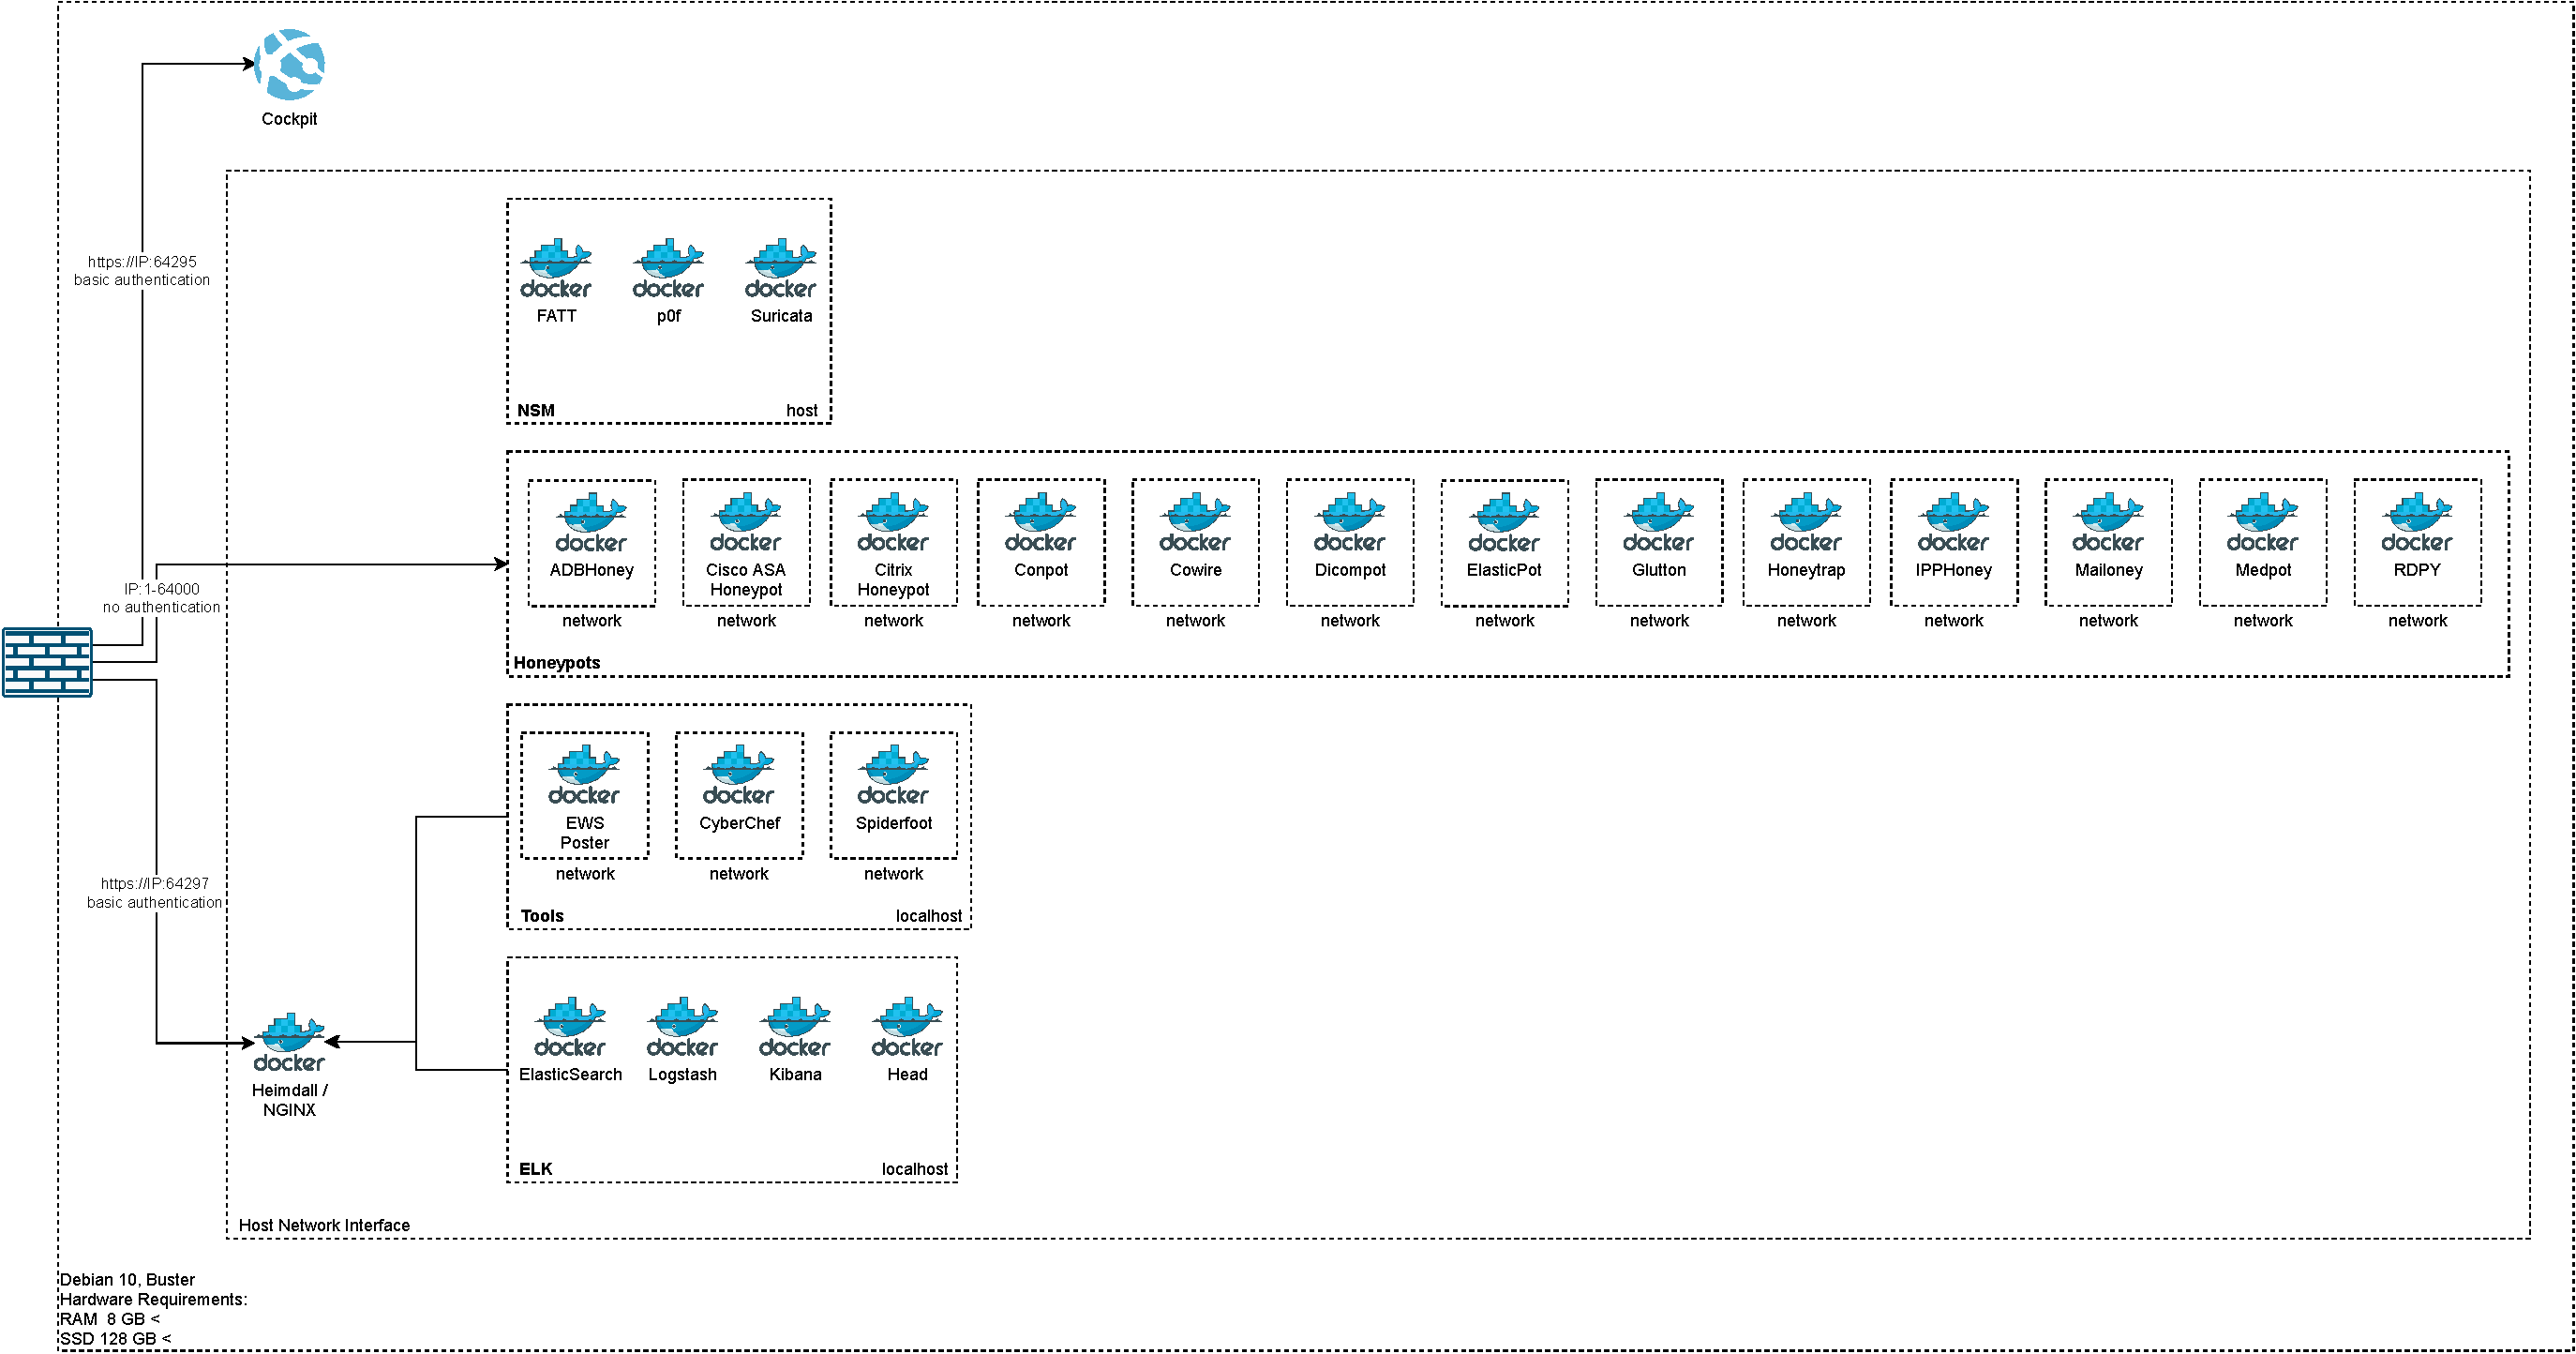
\includegraphics[width=\textwidth]{figures/tpot-architecture.pdf}
    \caption[T-Pot architecture]{T-Pot architecture derived from \cite{tpot}. Honeypots are encapsulated in their own network. NSM runs on the host network, and thus, receives every packet. ELK and tools run on localhost, and are accessible through NGINX.}
    \label{fig:overview-tpot}
\end{sidewaysfigure}

\subsubsection{Honeypots}

Followingly, all available components will be explained, albeit the sheer quantity of it.
In addition, \autoref{tab:overview-honeypots} gives a quick overview of all available honeypots in conjunction with
\begin{enumerate*}[label=(\roman*)]
    \item the port they are running on,
    \item thier interation level, and
    \item a short decription
\end{enumerate*}.

\textbf{ADBHoney} \cite{adbhoney2021} is a low interaction \ac{adb} honeypot over TCP/IP.
The importance of it lies in the \ac{adb} protocol that is used to debug and push content to the device.
However, unlike USB it does not support any kind of ample mechanisms of authentication and protection.
By exposing the \ac{adb} service over any port, an adversary could connect and exploit it.
ADBHoney is designed to catch malware that has been pushed onto devices.

\textbf{Cisco \ac{asa}} \cite{cymmetria2018} is a low interaction honeypot that detects CVE-2018-0101\cite{CVE-2018-0101}.
It is a vulnerability that could allow an unauthenticated, remote attacker to cause a reload of the affected system or to remotely execute code.
This can be achieved by flooding a webvpn-configured interface with crafted XML packets.
Consequently, the attacker obtain full control by executing arbitrary code.

\textbf{Citrix \ac{adc} honeypot} \cite{citrixhoneypot2020} detects and logs CVE-2019-19781\cite{CVE-2019-19781} scans and exploitation attempts.
This vulnerability allows adversaries to perform directory traversal attacks.
Files are accessible by path strings to denote the file or directory.
In addition, some file systems include special character to easily traverse the hierarchy.
Attackers take advantage of it by combining special characters in order to get access to restricted areas. \cite{flanders2019}

\textbf{Conpot} \cite{conpot2021} is a low interaction industrial honeypot for \ac{ics}, and \ac{scada}.
It provides a variety of different common industrial control protocols.
An adversary should be tricked by the complex infrastructure, and lure him into attacks.
In addition, a custom human machine interface can be conntected to increase the attack surface.
By randomly delaying the response time, conpot tries to emulate a real machine handling a certain amount of load.

\textbf{Cowrie} \cite{cowire2021} is a medium to high interaction SSH and Telnet honeypot.
It offers to log brute-force attacks and shell interactions with attackers.
In medium interaction mode cowire emulates a UNIX shell in Python, whereas in high interaction mode it proxies all commands to another system.

\textbf{DDoSPot} \cite{ddosspot2021} is a low interaction honeypot to log and detect UDP-based \ac{ddos} attacks.
It is used as a platform to support various plugins for different honeypot services, and servers.
Currently, it supports DNS, NTP, SSDP, CHARGEN, and random/mock UDP server.

\textbf{Dicompot} \cite{dicompot2021} is a low interaction honeypot for the \ac{dicom} protocol.
As other honeypots before, it mocks a \ac{dicom} server in Go to collect logs and detect attacks.

\textbf{Dionaea} \cite{dionaea2021} is a medium interaction honeypot that tries to capture malware copies by exposing services.
It supports a vast variety of protocols such as FTP, SMB, and HTTP.
Several modules can be integrated to work with Dionaea such as VirusTotal for further malware results.

\textbf{Elasticpot} \cite{elasticpot2021} is a low interaction honeypot for elasticsearch, a search engine based on the Lucene library.

\textbf{Glutton} \cite{glutton2021} is a generic low interaction honeypot that works as a MitM for SSH and TCP.
However, lacking documentation does not provide a deeper inside of this honeypot.

\textbf{Heralding} \cite{heralding2021} is a credential catching honeypot for protocols like FTP, Telnet, SSH, HTTP, or IMAP.

\textbf{HoneyPy} \cite{honeysap2021} is a low to medium interaction honeypot that supports several protocols such as UDP, or TCP.
New protocols can be added by writing a custom plugin for it.
HoneyPy should give the freedom of easily deploying and extending honeypots.

\textbf{HoneySAP} \cite{honeysap2021} is a low interaction honeypot tailored for SAP services.

\textbf{HoneyTrap} \cite{honeytrap2021} is a low interaction honeypot network security tool.
As stated by \citet*{honeytrap2021}, HoneyTrap is vulnerable to buffer overflow attacks.

\textbf{IPPHoney} \cite{ipphoney2021} is a low interaction \ac{ipp} honeypot.

\textbf{Mailoney} \cite{mailoney2021} is a low interaction SMTP honeypot written in Python.

\textbf{MEDpot} \cite{medpot2021} is a low interaction honeypot focused on \ac{fhir}.
It is a standard decription data format to transfer and exchange medical health records.

\textbf{RDPY} \cite{rdpy2021} is a low interaction honeypot of the Microsoft \ac{rdp} written in Python.
It features client and server side, and it based on the event driven network engine Twisted.
It supports authentication over SSL and NLA.

\textbf{SNARE and TANNER} \cite{snare2021, tanner2021} is a honeypot project.
SNARE is an abbreviation for Super Next generation Advanced Reactive honEypot.
It is a successor of Glastopf, a web application sensor.
In addition, it supports the feature of converting existing webpages into attack surfaces.
TANNER \cite{tanner2021} can be seen as SNARES's brain.
Whenever a request has been sent to SNARE, TANNER decides how the response should like.

\subsubsection{Tools}

T-Pot integrates tools to screen network traffic.

\textbf{FATT} \cite{fatt2021} is used to extract metadata and fingerprints such as JA3 \cite{ja32021} and HASSH \cite{hassh2021} from captured packets.
JA3 is a method for \enquote{creating SSL/TLS client fingerprints} whereas HASSH is a \enquote{network fingerprinting standard which can be used to identify specific client and server SSH implementations}.
In addition, it features live network traffic.
As noted by the author, FATT is based on a python wrapper for tshark, namely pyshark, and thus having performance downturns.
T-Pot applies FATT on every request made on the host network.

\textbf{Spiderfoot} \cite{spiderfoot2021} is an open source intelligence automation tool that helps to screen targets to get information about what is exposed over the Internet.
It can target different entities such as IP address, domain, hostname or network subnet.
In addition, it features more than 200 modules that can be integrated as an extension.
T-Pot uses it to scan defensively and thus not include any other module.

\textbf{Suricata} \cite{suricata2021} is a \enquote{a high performance \ac{ids}, \ac{ips} and \ac{nsm} engine}.
T-Pot lets suricata analyze and assess any request made on the host network.

\textbf{p0f} \cite{p0f2021} is a fingerprinting tool that uses passive traffic fingerprinting mechanisms to check TCP/IP communications.
T-Pot lets p0f passively check any request made on the host network.

\textbf{Endlessh} \cite{endlessh2021} is a SSH server that sends an endless, random SSH banner.
The key idea is to lock up SSH clients that try to connect to the SSH server.
It lowers the transcation speed by intentionally inserting delays.
Due to connection establishing before cryptographic exchange, this module does not require any cryptographic libraries.

\textbf{HellPot} \cite{hellpot2021} is a \enquote{endless honeypot}.
Connecting to this honeypot results in a memory overflow.
Its key idea is to send an endless stream of data to the attacker until its memory, or storage runs out.

\begin{sidewaystable}
    \centering
    \caption[Overview honeypots of T-Pot]{Overview of all available honeypots and tools of T-Pot with interaction level, port, and a short description. Ports are marked with either TCP or UDP, if a port misses any definition, both TCP and UDP are allowed.}
    \begin{tabularx}{\linewidth}{l|XlX}
        \toprule
        \textsc{Honeypots}                        & \multicolumn{3}{c}{}                                                                                                                                                                                                            \\
                                                  & \textbf{Port}                                                                                               & \textbf{Interaction-level} & \textbf{Description}                                                                 \\
        \hline
        ADBHoney \cite{adbhoney2021}              & 5555/tcp                                                                                                    & low                        & \ac{adb} protocol honeypot                                                           \\
        Cisco ASA \cite{cymmetria2018}            & 5000/udp, 8443/tcp                                                                                          & low                        & honeypot for CVE-2018-0101\cite{CVE-2018-0101} detection                             \\
        Citrix honeypot \cite{citrixhoneypot2020} & 443/tcp                                                                                                     & low                        & detects and logs CVE-2019-19781\cite{CVE-2019-19781} scans and exploitation attempts \\
        Conpot \cite{conpot2021}                  & 80, 102, 161, 502, 623, 1025, 2404, \newline 10001, 44818, 47808, 50100                                     & low                        & industrial honeypot for \ac{ics}, and \ac{scada}                                     \\
        Cowrie \cite{cowire2021}                  & 2222, 23                                                                                                    & high                       & SSH and Telnet honeypot                                                              \\
        DDoSPot \cite{ddosspot2021}               & 1112/tcp                                                                                                    & low                        & log and detect UDP-based \ac{ddos} attacks                                           \\
        Dicompot \cite{dicompot2021}              & 1112/tcp                                                                                                    & medium                     & honeypot for the \ac{dicom} protocol                                                 \\
        Dionaea \cite{dionaea2021}                & 21, 42, 69/udp, 8081, 135, 443, 445, \newline 1433, 1723, 1883, 1900/udp, \newline 3306, 5060/udp, 5061/udp & low                        & capture malware copies                                                               \\
        Elasticpot \cite{elasticpot2021}          & 9200                                                                                                        & low                        & honeypot for elasticsearch                                                           \\
        Glutton \cite{glutton2021}                & NFQ                                                                                                         & medium                     & MitM proxy for SSH and TCP                                                           \\
        Heralding \cite{heralding2021}            & 21, 22, 23, 25, 80, 110, 143, 443, \newline 993, 995, 1080, 5432, 5900                                      & low                        & credential catching honeypot                                                         \\
        HoneyPy \cite{honeysap2021}               & 7, 8, 2048, 2323, 2324, 4096, 9200                                                                          & low                        & extendable honeypot                                                                  \\
        HoneySAP \cite{honeysap2021}              & 3299/tcp                                                                                                    & low                        & honeypot for SAP services                                                            \\
        HoneyTrap \cite{honeytrap2021}            & NFQ                                                                                                         & medium                     & captures attacks via unknown protocols                                               \\
        IPPHoney \cite{ipphoney2021}              & 631                                                                                                         & low                        & \ac{ipp} honeypot                                                                    \\
        Mailoney \cite{mailoney2021}              & 25                                                                                                          & low                        & SMTP honeypot                                                                        \\
        MEDpot \cite{medpot2021}                  & 2575                                                                                                        & low                        & \ac{fhir} honeypot                                                                   \\
        RDPY \cite{rdpy2021}                      & 3389                                                                                                        & low                        & Microsoft \ac{rdp} honeypot                                                          \\
        SNARE/TANNER \cite{snare2021}             & 80                                                                                                          & low                        & web application honeypot                                                             \\
        \bottomrule
    \end{tabularx}
    \label{tab:overview-honeypots}
\end{sidewaystable}

\section{Results}
\label{sec:honeypots-heicloud}

Our T-Pot has been deployed for 3 weeks (from 22nd of September to 22nd of October) and collected in total $825539$ attacks.
Overall, RDPY ($49.15\%$), HoneyTrap ($32.01\%$), and Cowire ($11.97\%$) received most of the attacks with a total amount of $540398$ attacks.
\autoref{fig:overview-attacks} shows the distribution of honeypot attacks.
The total numbers are based on \autoref{tab:overview-honeypots-attacks}.
%As \citet{Kelly2021} states, the vast majority of attacks origin from bots\todo{more to bots}

\begin{figure}[h]
    \centering
    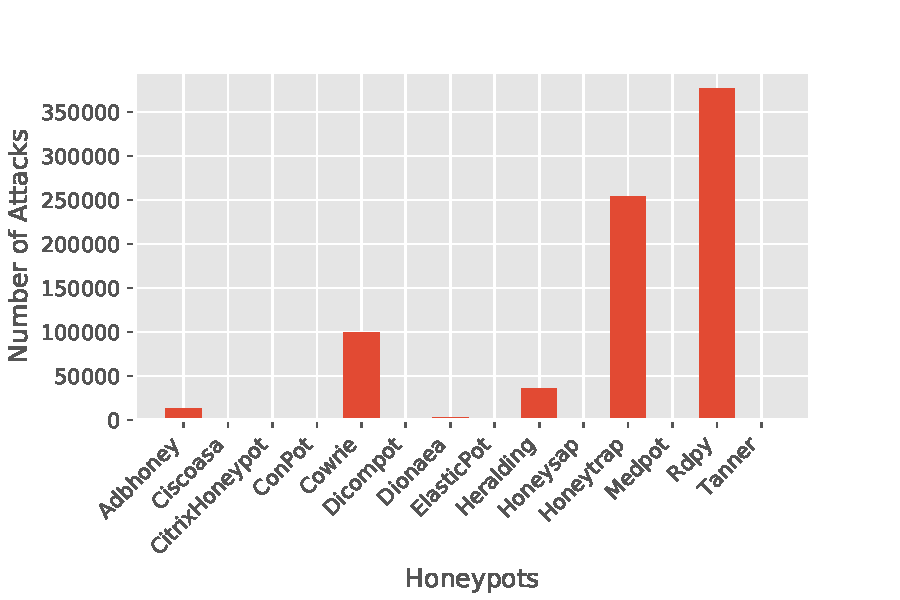
\includegraphics[width=\textwidth]{figures/tpot-overview-attacks.pdf}
    \caption[Distribution of honeypot attacks]{Distribution of honeypot attacks}
    \label{fig:overview-attacks}
\end{figure}

Noticeable is the large disparity of the previously mentioned attacks on \ac{aws}, \ac{gcp}, and Azure.
Especially for honeypots like Dionaea, it is shallow why so little attacks have been performed.
Therefore, we assume that packets run through a static filter. 
Heidelberg itself has a centralized packet filtering which indicates our assumption that certain ports or protocols are excluded.
To prove that, a \textsc{nmap} TCP SYN scan (\ipAddress{nmap -sS -A 129.206.5.74}) has been executed.
Our result clearly shows that port 20, resevered for FTP, is filtered although the access security explicitly allows it.
Based on this, most of the attacks on Dionaea are made throughout FTP, and thus, explains the total number of attacks.
Moreover, $96\%$ of IP addresses connected to Dionaea are known attackers, and $70\%$ were acquired on port 81, unofficially known for Tor routing.
Neither any malware or supicious payload could be identified.
Even with an \ac{acl} running in the background heiCLOUD received more attacks than ever.
We assume without packet filtering for FTP port 20, the real number might be even higher.
However, due to security concerns a temporarily exclude of this rule has been rejected.

\begin{figure}[h]
    \centering
    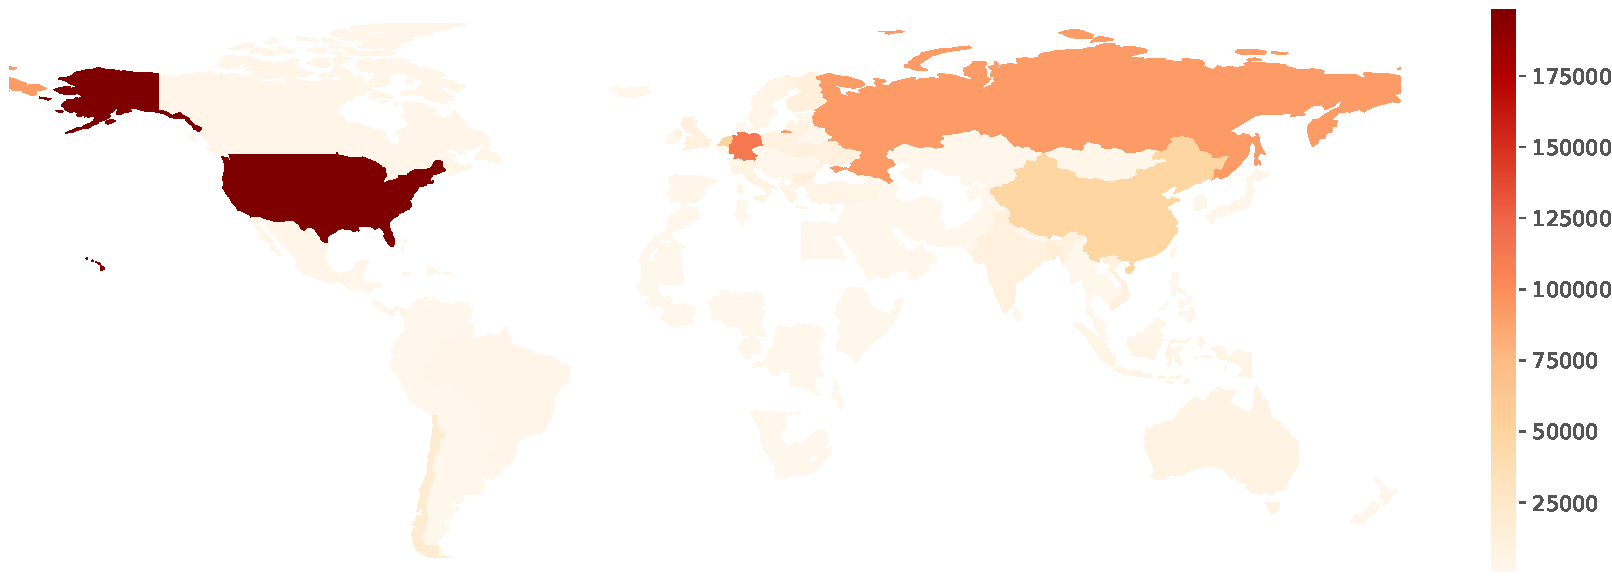
\includegraphics[width=\textwidth]{figures/tpot-overview-map.pdf}
    \caption[Attack distribution]{Attack distribution}
    \label{fig:attack-distribution}
\end{figure}

\autoref{fig:attack-distribution} indicates the geographical location of connections acquired to any honeypot.
Most attacks are originated from United States, Germany, Russia, and China.
Large security scans of DFN or BelWÜ pushes Germany on second place.
Therefore, Germany can be considered as negligible.
However, the geographical location merely indicates the last node of an IP address, and thus as stated by \citet{Kelly2021}, this information is insufficient to use.
Adversaries could use VPN or Tor to spoof their true location. 
adversaries are capable of disguising their fingerprint activities.

\begin{figure}[h]
    \centering
    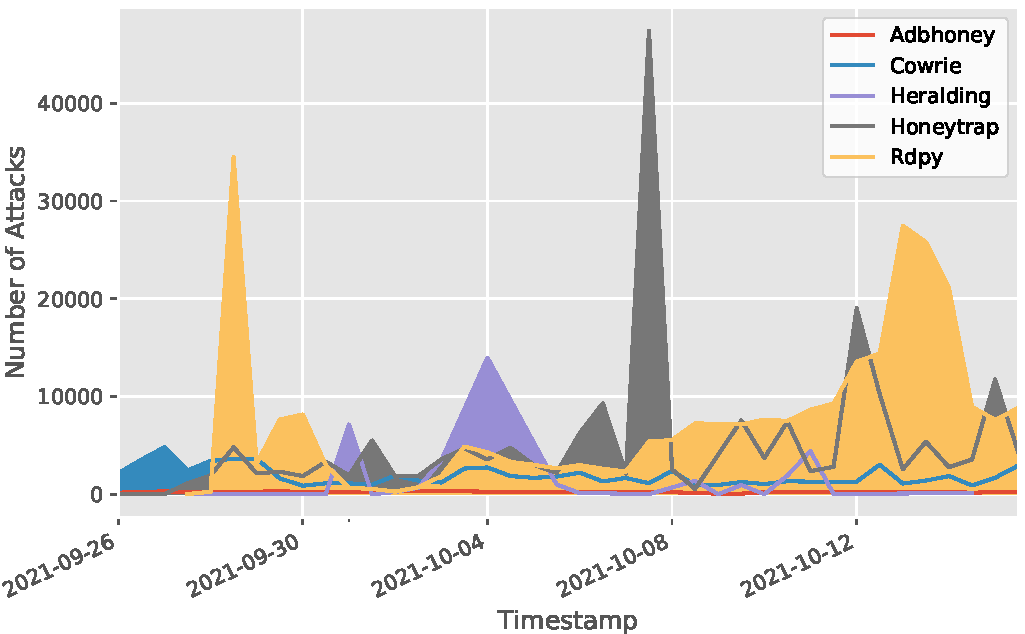
\includegraphics[width=\textwidth]{figures/tpot-attacks-histogram.pdf}
    \caption[Attack histogram]{Attack histogram}
    \label{tpot-overview-histogram}
\end{figure}

\autoref{tpot-overview-histogram} shows the timeline of attacks that are executed on our instance.
The high peak in the middle indicates a full \textsc{nmap} scan from Germany.

\begin{figure}[h]
    \centering
    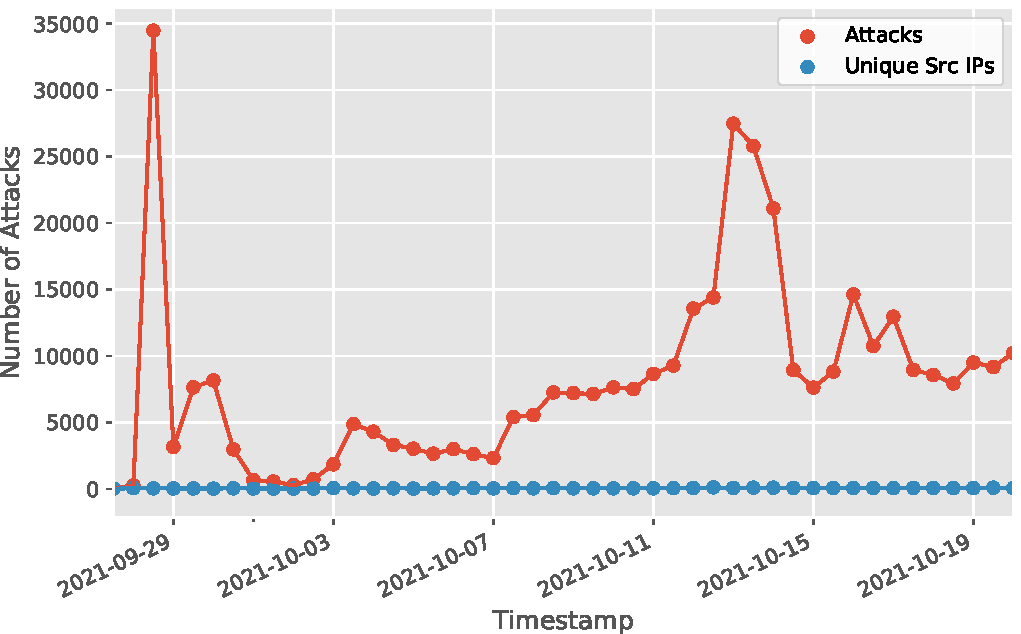
\includegraphics[width=\textwidth]{figures/tpot-rdpy-port.pdf}
    \caption[RDPY results]{RDPY results}
    \label{fig:rdpy-results}
\end{figure}

The results from \textbf{RDPY} 
We assume the skyrocketing number of attacks roots back to the Corona pandemic.
It resulted in an increase of screen sharing software 
\autoref{fig:rdpy-results} visualizes the results of RDPY.

\begin{figure}[h]
    \centering
    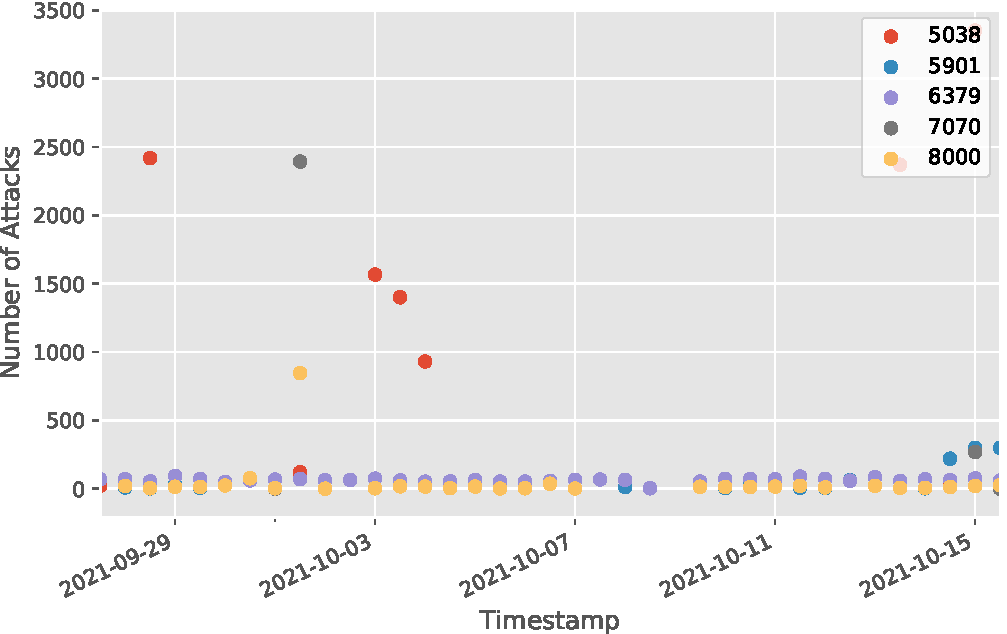
\includegraphics[width=\textwidth]{figures/tpot-honeytrap-port.pdf}
    \caption[Honeytrap results]{Honeytrap results}
    \label{fig:honeytrap-results}
\end{figure}

\textbf{Honeytrap}

\begin{figure}[h]
    \centering
    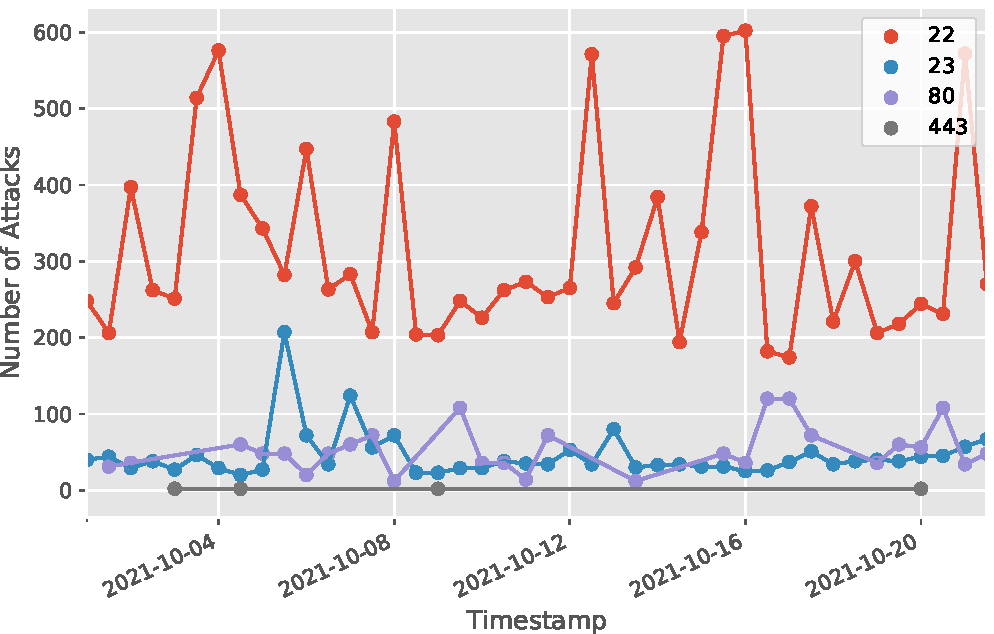
\includegraphics[width=\textwidth]{figures/tpot-cowire-port.pdf}
    \caption[Cowire results]{Cowire results}
    \label{fig:cowire}
\end{figure}

\textbf{Cowire} results in a high use of 

\begin{figure}[h]
    \centering

    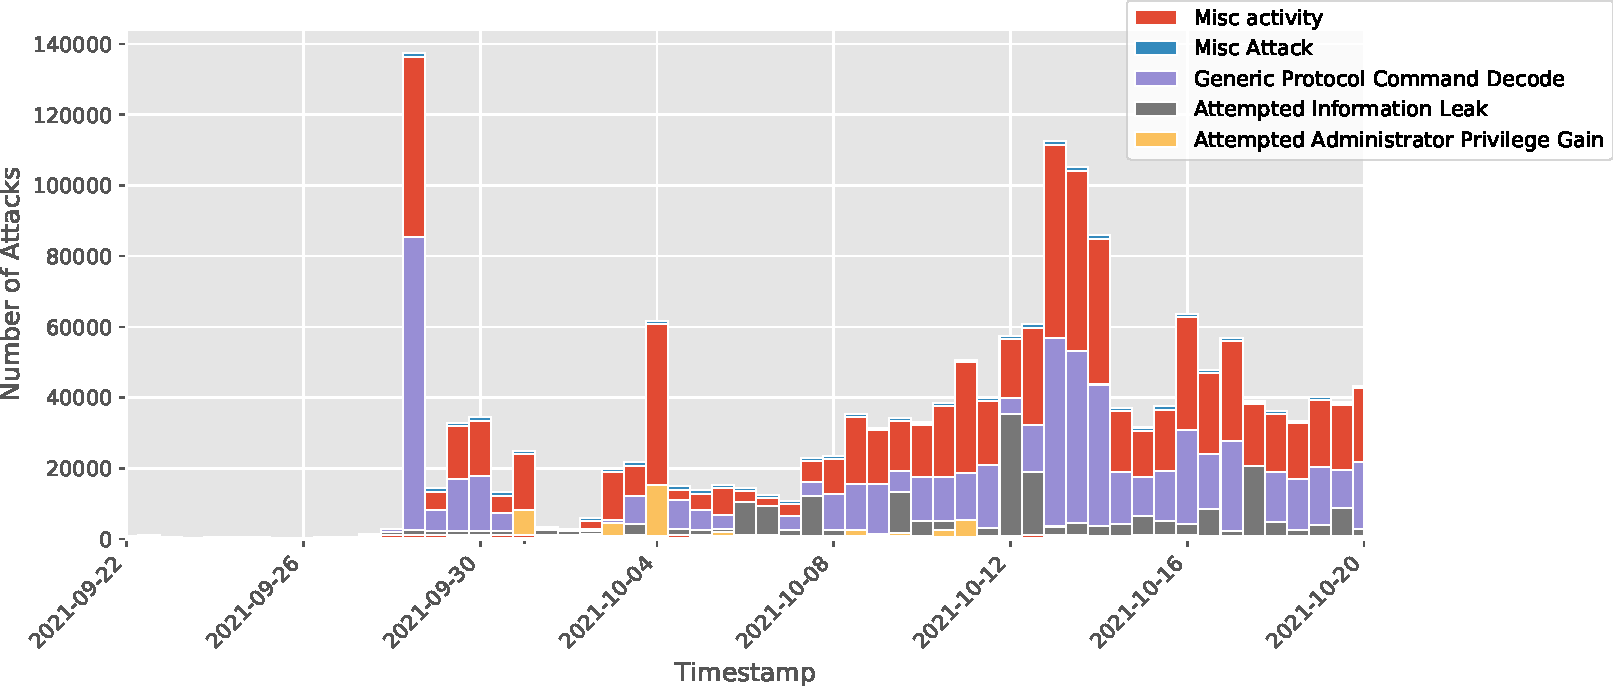
\includegraphics[width=\textwidth]{figures/tpot-suricata-alerts.pdf}
    \caption[Suricata results]{Suricata results}
    \label{fig:suricata-results}
\end{figure}

\textbf{Suricata}

Interestingly, zero-day exploits like the Apache vulnerability \cite{CVE-2021-42013} that came with version $2.49.0$ got registered in CVE on the 6th of October, and immediately used by attackers on the 15th of October.
Attackers could perform a remote code execution using path traversal attack when the CGI scripts of Apache are enabled.
This shows how fast attackers, most likely bots, adapt to new vulnerabilities in order to compromise more systems.

% Blockchain attacks

% Conclusion
We assume that attacks made by bots have increased significantly in the last years.
This might even route back to the Corona pandemic and the skyrocketing increase of Internet activities throughout home offices, more usage of screen sharing software, .

\begin{sidewaystable}
    \centering
    \caption[Overview of attacks on cloud providers]{Overview of attacks on heiCLOUD, AWS, GC and Azure. Only the top 10 most attacked honeypots are considered. \enquote{-} entails that a honeypot is not part of the top 10.}
    \begin{tabularx}{\linewidth}{l|XX|XX|XX|XX}
        \toprule
        \textsc{Honeypots}                        & \multicolumn{2}{c}{BASIS}             & \multicolumn{6}{c}{\textsc{comparision}}                                                                                                                                             \\
                                                  & \multicolumn{2}{c|}{\textsc{heicloud}} & \multicolumn{2}{c|}{\textsc{AWS}}        & \multicolumn{2}{c|}{\textsc{GC}} & \multicolumn{2}{c}{\textsc{Azure}}                                                                     \\
                                                  & \textbf{Number}                        & \textbf{Pct.}                            & \textbf{Number}                  & \textbf{Pct.}                      & \textbf{Number} & \textbf{Pct.} & \textbf{Number} & \textbf{Pct.} \\
        \hline
        ADBHoney \cite{adbhoney2021}              & $13586$                                & $1.65\%$                                 & 413                              & $0.13\%$                           & 2497            & $0.43\%$      & 442             & $0.13\%$      \\
        Cisco ASA \cite{cymmetria2018}            & $931$                                  & $0.11\%$                                 & 260                              & $0.08\%$                           & 750             & $0.13\%$      & 134             & $0.04\%$      \\
        Citrix honeypot \cite{citrixhoneypot2020} & $1480$                                 & $0.18\%$                                 & -                                & -                                  & -               & -             & -               & -             \\
        Conpot \cite{conpot2021}                  & $807$                                  & $0.10\%$                                 & -                                & -                                  & -               & -             & -               & -             \\
        Cowrie \cite{cowire2021}                  & $98813$                                & $11.97\%$                                & 4503                             & $1.46\%$                           & 297818          & $51.25\%$     & 9012            & $2.64\%$      \\
        DDoSPot \cite{ddosspot2021}               & $0$                                    & $0\%$                                    & -                                & -                                  & -               & -             & -               & -             \\
        Dicompot \cite{dicompot2021}              & $27$                                   & $0\%$                                    & -                                & -                                  & -               & -             & -               & -             \\
        Dionaea \cite{dionaea2021}                & $3293$                                 & $0.40\%$                                 & 288075                           & $93.49\%$                          & 162570          & $27.98\%$     & 308102          & $90.42\%$     \\
        Elasticpot \cite{elasticpot2021}          & $531$                                  & $0.06\%$                                 & -                                & -                                  & -               & -             & -               & -             \\
        Glutton \cite{glutton2021}                & $0$                                    & $0\%$                                    & 11878                            & $3.85\%$                           & 84375           & $15.52\%$     & 17256           & $5.06\%$      \\
        Heralding \cite{heralding2021}            & $35843$                                & $4.34\%$                                 & 1885                             & $0.61\%$                           & 12255           & $2.11\%$      & 3370            & $0.99\%$      \\
        HoneyPy \cite{honeysap2021}               & $0$                                    & $0\%$                                    & 172                              & $0.06\%$                           & 2149            & $0.37\%$      & 497             & $0.15\%$      \\
        HoneySAP \cite{honeysap2021}              & $18$                                   & $0\%$                                    & -                                & -                                  & -               & -             & -               & -             \\
        HoneyTrap \cite{honeytrap2021}            & $264264$                               & $32.01\%$                                & -                                & -                                  & -               & -             & -               & -             \\
        IPPHoney \cite{ipphoney2021}              & $0$                                    & $0\%$                                    & -                                & -                                  & -               & -             & -               & -             \\
        Mailoney \cite{mailoney2021}              & $0$                                    & $0\%$                                    & 720                              & $0.23\%$                           & 9419            & $1.62\%$      & 146             & $0.04\%$      \\
        MEDpot \cite{medpot2021}                  & $3$                                    & $0\%$                                    & -                                & -                                  & -               & -             & -               & -             \\
        RDPY \cite{rdpy2021}                      & $405742$                               & $49.15\%$                                & 100                              & $0.03\%$                           & 7916            & $1.36\%$      & 1463            & $0.43\%$      \\
        SNARE/TANNER \cite{snare2021}             & $201$                                  & $0.02\%$                                 & 138                              & $0.04\%$                           & 1367            & $0.24\%$      & 313             & $0.09\%$      \\
        \hline
        \textsc{In total}                         & $825539$                               & $100\%$                                  & 308144                           & $100\%$                            & 581116          & $100\%$       & 340735          & $100\%$       \\
        \bottomrule
    \end{tabularx}
    \label{tab:overview-honeypots-attacks}
\end{sidewaystable}

\section{Discussion}

As recently investigated by \citet{vetterl2020}, fingerprinting honeypots is becoming easier due to a fatal flaw in the underlying protocol implementation.
\citet{vetterl2020} states that attackers always try to prevent their methods, exploits and tools to be disclosed.
Therefore detecting honeypots before attack them to avoid disclosing potential skills is a strong motivation for black hats.


\section{Summary}

In this chapter we have
